%% Figure from MATH 556 notes, section 49 (Lecture 22). board sketch (Lecture 22), redrawn.
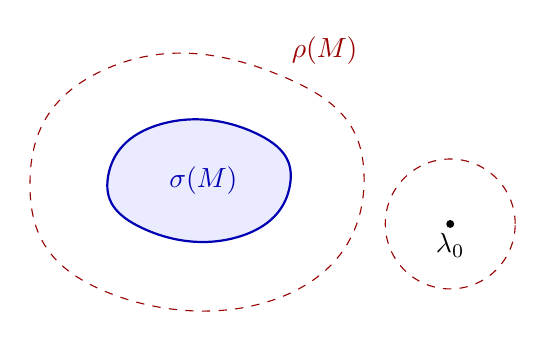
\begin{tikzpicture}[scale=1.1, >=stealth]
    \draw[dashed, red!60!black] plot[smooth cycle, tension=0.8] coordinates {(-2.1,0.1) (-1.2,1.35) (0.7,1.3) (1.75,0.2) (0.9,-1.25) (-1.3,-1.2)};
    \draw[thick, blue!70!black, fill=blue!8] plot[smooth cycle, tension=0.8] coordinates {(-1.2,0.1) (-0.6,0.7) (0.5,0.6) (0.9,0.0) (0.3,-0.6) (-0.8,-0.5)};
    \node[blue!70!black] at (-0.1,0.05) {$\sigma(M)$};
    \node[red!60!black] at (1.3,1.55) {$\rho(M)$};
    \fill (2.75,-0.45) circle (1.3pt) node[below] {$\lambda_0$};
    \draw[dashed, red!60!black] (2.75,-0.45) circle (0.75);
\end{tikzpicture}
